\documentclass[11pt,a4paper]{article}
\usepackage[margin=2.3cm]{geometry}
\usepackage[T1]{fontenc}
\usepackage{textcomp}
\input{glyphtounicode}
\pdfgentounicode=1
\usepackage{lmodern}
\usepackage{amsmath}
\usepackage{xcolor}
\usepackage{listings}
\usepackage{tcolorbox}
\tcbuselibrary{breakable}
\usepackage{booktabs}
\usepackage{array}
\usepackage{tikz}
\usetikzlibrary{decorations.pathreplacing}
\usepackage{float}
\usepackage{graphicx}
\graphicspath{{images/}}
\usepackage{hyperref}
\hypersetup{colorlinks=true, linkcolor=blue!50!black, citecolor=green!40!black}

\usepackage{accsupp}
% line numbers are drawn but excluded from copied text
\newcommand{\nocopy}[1]{\BeginAccSupp{method=escape,ActualText={}}#1\EndAccSupp{}}
\lstset{
  language=C, basicstyle=\ttfamily\small, keywordstyle={}, commentstyle={}, stringstyle={},
  numbers=left, numberstyle=\footnotesize\nocopy, numbersep=10pt, xleftmargin=2.4em,
  frame=none, columns=fullflexible, keepspaces=true, upquote=true, showstringspaces=false,
  breaklines=true, captionpos=b, aboveskip=1em, belowskip=0.8em
}
\lstdefinestyle{sh}{language=bash, numbers=none, xleftmargin=2.4em}
\renewcommand{\lstlistingname}{Listing}
% code names in the text: grey monospace
\let\origtexttt\texttt
\renewcommand{\texttt}[1]{\textcolor{black!60}{\origtexttt{#1}}}

\newtcolorbox{keyidea}{colback=blue!4, colframe=blue!45!black, title=Key ideas, fonttitle=\bfseries\small}
\newtcolorbox{experiment}{breakable, colback=orange!5, colframe=orange!70!black, title=Experiment, fonttitle=\bfseries\small}
\title{\textbf{OpenMP GPU Offloading: \texttt{target}, \texttt{map} and \texttt{teams distribute}}\\[4pt]\large Lesson 30: running loops on the GPU and moving data to it}
\author{Gustavo Lozano}
\date{November 2026}

\begin{document}
\maketitle

\noindent\textit{\small Source: Deakin \& Mattson~\cite{dm}, Ch.~3 (Running Parallel Code on a GPU)
and Ch.~4 (Memory Movement).}

\section{The idea}
The CPU (the \emph{host}) and the GPU (the \emph{device}) have separate memories joined by
the PCIe bus (Figure~\ref{fig:hw}). A loop on the GPU can only use data that is in GPU
memory, so offloading has two parts:
\begin{itemize}
  \item \texttt{target}: run this code on the device;
  \item \texttt{map}: copy these arrays between host and device memory.
\end{itemize}
The GPU memory is about 3 times faster than the CPU memory, but the PCIe bus is about 3 times
\emph{slower}. A kernel only gains if its data crosses the bus rarely.

\begin{figure}[H]
\centering
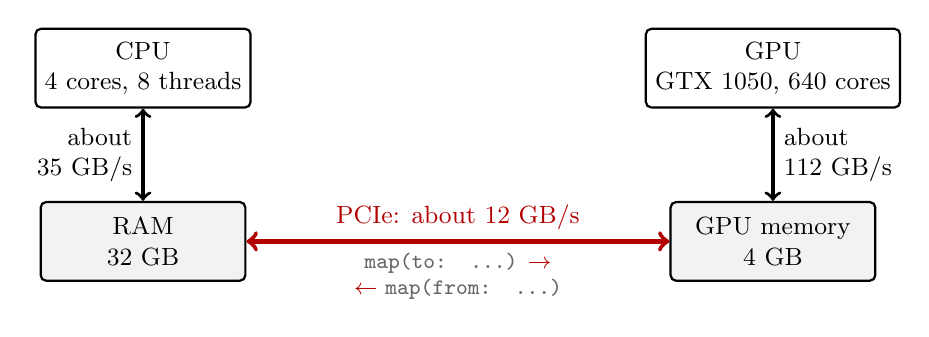
\begin{tikzpicture}[font=\small, box/.style={draw, thick, rounded corners=2pt, minimum
  height=1cm, align=center}]
  \node[box, minimum width=2.6cm] (cpu) at (0,0) {CPU\\ 4 cores, 8 threads};
  \node[box, minimum width=2.6cm, fill=black!5] (ram) at (0,-2.2) {RAM\\ 32 GB};
  \node[box, minimum width=2.6cm] (gpu) at (8,0) {GPU\\ GTX 1050, 640 cores};
  \node[box, minimum width=2.6cm, fill=black!5] (vram) at (8,-2.2) {GPU memory\\ 4 GB};
  \draw[<->, very thick] (cpu) -- node[left, align=right] {about\\ 35 GB/s} (ram);
  \draw[<->, very thick] (gpu) -- node[right, align=left] {about\\ 112 GB/s} (vram);
  \draw[<->, line width=1.6pt, red!70!black] (ram.east) -- node[above] {PCIe: about 12 GB/s}
     node[below, align=center, font=\footnotesize] {\texttt{map(to: ...)} $\rightarrow$\\
     $\leftarrow$ \texttt{map(from: ...)}} (vram.west);
\end{tikzpicture}
\caption{Host and device on this laptop. Approximate peak bandwidths.}
\label{fig:hw}
\end{figure}

\section{The constructs}
\paragraph{Running a loop on the GPU.} A GPU has many small cores grouped in
\emph{streaming multiprocessors}. OpenMP maps this to two levels (Figure~\ref{fig:teams}):
\begin{lstlisting}[numbers=none]
#pragma omp target teams distribute parallel for
for (long i = 0; i < n; i++) ...
\end{lstlisting}
\begin{itemize}
  \item \texttt{target}: the loop runs on the device;
  \item \texttt{teams}: start a league of teams (one or more per multiprocessor);
  \item \texttt{distribute}: split the iterations among the teams;
  \item \texttt{parallel for}: split each team's iterations among its threads.
\end{itemize}
Threads of different teams cannot synchronize; \texttt{reduction} still works across all of
them.

\begin{figure}[H]
\centering
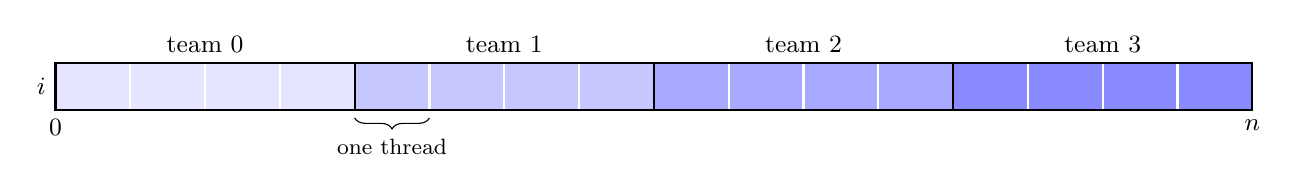
\begin{tikzpicture}[font=\small, x=0.95cm]
  \draw[thick] (0,0) rectangle (16,0.6);
  \node[left] at (0,0.3) {$i$};
  \foreach \t/\c in {0/10,1/22,2/34,3/46} {
    \fill[blue!\c] (4*\t,0) rectangle ++(4,0.6);
    \foreach \k in {1,2,3} \draw[white, thick] (4*\t+\k,0) -- ++(0,0.6);
    \draw[thick] (4*\t,0) rectangle ++(4,0.6);
    \node[above] at (4*\t+2,0.6) {team \t};
  }
  \node[below] at (0,0) {0}; \node[below] at (16,0) {$n$};
  \draw[decorate, decoration={brace, mirror, amplitude=4pt}] (4,-0.1) -- (5,-0.1)
     node[midway, below=4pt, font=\footnotesize] {one thread};
\end{tikzpicture}
\caption{\texttt{distribute} gives each team a block of iterations; \texttt{parallel for}
splits the block among the team's threads (here 4 teams of 4 threads; a GPU uses hundreds of
teams of up to 1024 threads each).}
\label{fig:teams}
\end{figure}

\paragraph{Moving data.} Pointers to the heap need explicit array sections
\texttt{x[first:length]}:
\begin{center}
\small
\begin{tabular}{@{}ll@{}}
\toprule
map type & copy \\ \midrule
\texttt{to}     & host $\rightarrow$ device when the region starts \\
\texttt{from}   & device $\rightarrow$ host when the region ends \\
\texttt{tofrom} & both (the default for arrays) \\
\texttt{alloc}  & no copy, only space on the device \\
\bottomrule
\end{tabular}
\end{center}
A \texttt{target data} region keeps arrays on the device across many \texttt{target} regions.
Inside it, a \texttt{map} for an array that is already present copies nothing. So the same
function can be called with or without copies (Listing~\ref{lst:gpu}, lines 110--118).

\paragraph{Where did it run?} If there is no usable GPU, a \texttt{target} region silently runs
on the host. The function \texttt{omp\_is\_initial\_device()} returns 1 on the host and 0 on
the device (lines 90--94). With the environment variable\\
\texttt{OMP\_TARGET\_OFFLOAD=MANDATORY} the program stops with an error instead of falling
back.

\section{The code}
The program runs \texttt{axpy} ($y \leftarrow a x + y$) and a dot product $s = x\cdot y$ 20
times in three ways: on the CPU, on the GPU copying $x$ and $y$ on every call, and on the GPU
inside a \texttt{target data} region. Each version checks the exact result. Bandwidth is
counted as 40 bytes per element and iteration (\texttt{axpy} reads $x,y$ and writes $y$;
the dot product reads $x,y$).

\begin{lstlisting}[caption={\textbf{\origtexttt{target\_axpy\_dot.c}} -- \origtexttt{axpy} and dot product on the CPU and on the GPU, with and without \origtexttt{target data}.}, label={lst:gpu}]
/*
 * target_axpy_dot.c -- OpenMP Lesson 30: offloading to the GPU with
 * target, map and teams distribute parallel for.
 * Source: Deakin & Mattson (2023), Ch. 3 (target construct) and Ch. 4 (map).
 *
 * Kernels: y = a*x + y (axpy) and s = x.y (dot), run NITER times,
 *   cpu      : parallel for on the CPU threads
 *   gpu map  : every call copies x and y between CPU and GPU memory
 *   gpu data : x and y are copied once (target data); the calls reuse them
 *
 * Compile:  clang -O2 -fopenmp --offload-arch=sm_61 \
 *                 -o target_axpy_dot target_axpy_dot.c
 * Run:      ./target_axpy_dot [log2 n]
 */

#include <stdio.h>
#include <stdlib.h>
#include <omp.h>

#define NITER 20

/* ---- CPU ---------------------------------------------------------------- */
static void axpy_cpu(long n, double a, const double *x, double *y)
{
    #pragma omp parallel for
    for (long i = 0; i < n; i++)
        y[i] += a * x[i];
}

static double dot_cpu(long n, const double *x, const double *y)
{
    double s = 0.0;
    #pragma omp parallel for reduction(+: s)
    for (long i = 0; i < n; i++)
        s += x[i] * y[i];
    return s;
}

/* ---- GPU: the loop runs on the device; map says what to copy ------------ */
static void axpy_gpu(long n, double a, const double *x, double *y)
{
    #pragma omp target teams distribute parallel for \
            map(to: x[0:n]) map(tofrom: y[0:n])
    for (long i = 0; i < n; i++)
        y[i] += a * x[i];
}

static double dot_gpu(long n, const double *x, const double *y)
{
    double s = 0.0;
    #pragma omp target teams distribute parallel for reduction(+: s) \
            map(to: x[0:n], y[0:n]) map(tofrom: s)
    for (long i = 0; i < n; i++)
        s += x[i] * y[i];
    return s;
}

/* ---- helpers ------------------------------------------------------------ */
static void init(long n, double *x, double *y)
{
    for (long i = 0; i < n; i++) { x[i] = 1.0; y[i] = 2.0; }
}

/* exact result after NITER steps with a = 0.5: y = 2 + 0.5*NITER, s = n*y */
static const char *check(long n, const double *y, double s)
{
    double yk = 2.0 + 0.5 * NITER;
    for (long i = 0; i < n; i++)
        if (y[i] != yk) return "NO";
    return s == (double)n * yk ? "yes" : "NO";
}

static void report(const char *name, long n, double t, const double *y, double s)
{
    double ms = 1e3 * t / NITER;                      /* per iteration          */
    double gbs = 40.0 * n / (t / NITER) / 1e9;        /* 40 bytes per element   */
    printf("%-9s: %8.2f ms/iter  %7.1f GB/s   correct: %s\n",
           name, ms, gbs, check(n, y, s));
}

int main(int argc, char **argv)
{
    long n = 1L << (argc > 1 ? atoi(argv[1]) : 25);   /* 2^25 doubles = 256 MiB */
    const double a = 0.5;
    double *x = malloc(n * sizeof(double));
    double *y = malloc(n * sizeof(double));
    double s = 0.0, t;

    /* 1. Where does a target region run? (also starts up the GPU) */
    int on_host = 1;
    #pragma omp target map(from: on_host)
    on_host = omp_is_initial_device();
    printf("devices: %d   target region ran on: %s\n",
           omp_get_num_devices(), on_host ? "CPU (host)" : "GPU (device)");
    printf("n = %ld doubles (%.0f MiB per vector), %d iterations\n",
           n, n * 8.0 / (1 << 20), NITER);

    /* 2. CPU */
    init(n, x, y);
    t = omp_get_wtime();
    for (int k = 0; k < NITER; k++) { axpy_cpu(n, a, x, y); s = dot_cpu(n, x, y); }
    report("cpu", n, omp_get_wtime() - t, y, s);

    /* 3. GPU, copies on every call */
    init(n, x, y);
    t = omp_get_wtime();
    for (int k = 0; k < NITER; k++) { axpy_gpu(n, a, x, y); s = dot_gpu(n, x, y); }
    report("gpu map", n, omp_get_wtime() - t, y, s);

    /* 4. GPU, data kept on the device: inside target data the maps in
          axpy_gpu and dot_gpu find x and y already present: no copies */
    init(n, x, y);
    t = omp_get_wtime();
    #pragma omp target data map(to: x[0:n]) map(tofrom: y[0:n])
    {
        for (int k = 0; k < NITER; k++)
            { axpy_gpu(n, a, x, y); s = dot_gpu(n, x, y); }
    }   /* y is copied back here, once */
    report("gpu data", n, omp_get_wtime() - t, y, s);

    free(x); free(y);
    return 0;
}
\end{lstlisting}

\begin{lstlisting}[style=sh]
clang -O2 -fopenmp --offload-arch=sm_61 -o target_axpy_dot target_axpy_dot.c
OMP_TARGET_OFFLOAD=MANDATORY ./target_axpy_dot
\end{lstlisting}
\texttt{sm\_61} is the compute capability of the GTX 1050. If Clang cannot find CUDA, add
the option \texttt{-{}-cuda-path=/opt/cuda} to the compile line.

\begin{keyidea}
\begin{itemize}
  \item \texttt{target teams distribute parallel for}: the loop runs on the GPU, split over
        teams and then over the threads of each team.
  \item \texttt{map} copies data over PCIe, the slowest link in the machine.
  \item \texttt{target data} keeps arrays on the GPU; maps of present data copy nothing.
  \item Check where the code ran with \texttt{omp\_is\_initial\_device()}, and run with\\
        \texttt{OMP\_TARGET\_OFFLOAD=MANDATORY} so that a missing GPU is an error.
\end{itemize}
\end{keyidea}

\section{The experiment}
\begin{experiment}
\textbf{Question:} where does the time go when a loop is offloaded?

Run the program three times:
\begin{lstlisting}[style=sh]
OMP_TARGET_OFFLOAD=MANDATORY ./target_axpy_dot
OMP_TARGET_OFFLOAD=MANDATORY ./target_axpy_dot 27
OMP_TARGET_OFFLOAD=DISABLED  ./target_axpy_dot
\end{lstlisting}

\textbf{What to observe and answer.}
\begin{enumerate}
  \item The first line must say \texttt{GPU (device)}. What does the third run print, and
        why are the three timings then almost equal?
  \item Why is \texttt{gpu map} slower than \texttt{cpu}? How many bytes cross the PCIe bus
        per iteration?
  \item How much faster is \texttt{gpu data} than \texttt{cpu}? Compare with the ratio of the
        memory bandwidths in Figure~\ref{fig:hw}.
\end{enumerate}
\end{experiment}

\paragraph{Answers (read after trying).}

\noindent(1)~With \texttt{DISABLED} every \texttt{target} region runs on the host: the program
prints \texttt{CPU (host)}, and all three versions are CPU loops reading the same RAM.

\noindent(2)~Per iteration \texttt{axpy} copies $x$ and $y$ in and $y$ out, and the dot product
copies $x$ and $y$ in: 5 vectors of 256\,MiB, about 1.3\,GB. At about 12\,GB/s that is about
0.1\,s per iteration, several times the CPU time. The GPU computes fast and then waits for the
bus.

\noindent(3)~\texttt{gpu data} moves the vectors only twice in total, so the time is the GPU
memory time. Both kernels are limited by memory bandwidth, so the speed-up should be close to
$112/35 \approx 3$. With $2^{27}$ elements (1\,GiB per vector) the result is the same per
element; the GPU memory still holds both vectors.

\paragraph{Next lesson.} Lesson 31: keeping data on the GPU across functions and many
iterations with \texttt{target enter data}, \texttt{exit data} and \texttt{update}.

\begin{thebibliography}{9}
\bibitem{dm} T.~Deakin and T.~G.~Mattson. \emph{Programming Your GPU with OpenMP: Performance
  Portability for GPUs}. MIT Press, Cambridge, MA, 2023.
\end{thebibliography}
\end{document}
